\documentclass[a4paper,12pt]{article}
\usepackage[T1]{fontenc}
\usepackage[polish]{babel}
\usepackage{amsfonts}
\usepackage{listings}
\usepackage{graphicx}
\usepackage{caption}
\usepackage{booktabs}
\usepackage{amssymb}
\usepackage{amsmath}
\usepackage[dvipsnames]{xcolor}
\usepackage[T1]{fontenc}
\usepackage[utf8]{inputenc}
\usepackage{subcaption} 
\usepackage{float}
\usepackage{geometry}
\geometry{margin=1in}
\usepackage{graphicx}
\usepackage{babel}
\usepackage{animate}
\usepackage{hyphenat}
\usepackage{url} 

\geometry{left=2cm, right=2cm, top=2cm, bottom=2cm}

% Ustawienia dla środowiska lstlisting
\lstset{ 
  language=Python,
  basicstyle=\footnotesize\ttfamily,
  numbers=left,
  numberstyle=\tiny,
  numbersep=5pt,
  frame=single,
  breaklines=true,
  backgroundcolor=\color{gray!10},
  captionpos=b,
  tabsize=2,
}

\title{Sprawozdanie z laboratorium 7 - Rozwiązania układów równań linowych}
\author{Hubert Miklas}
\date{13-05-2025}

\begin{document}

\maketitle

\section{Wstęp}

Tematem laboratorium było rozwiązywanie układów równań liniowych, korzystając z metody LU, rozkładu QR i inwersji macierzy.

\section{Treści zadań}


\begin{itemize}
    \item Napisz program, który:
    \begin{enumerate}
        \item Jako parametr pobiera rozmiar układu równań $n$
        \item Generuje macierz układu $A(n \times n)$ i wektor wyrazów wolnych $b(n)$
        \item Rozwiązuje układ równań $Ax = b$ na trzy sposoby:
        \begin{enumerate}
            \item poprzez dekompozycję LU macierzy $A$: $A = LU$;
            \item poprzez odwrócenie macierzy $A$: $x = A^{-1}b$, sprawdzić czy $AA^{-1} = I$ i $A^{-1}A = I$ (macierz jednostkowa);
            \item poprzez dekompozycję QR macierzy $A$: $A = QR$.
        \end{enumerate}
        \item Sprawdzić poprawność rozwiązania (tj. czy $Ax = b$)
        \item Zmierzyć całkowity czas rozwiązania układu.
        \item Porównać czasy z trzech sposobów: poprzez dekompozycję LU, poprzez \textbf{odwrócenie macierzy} i poprzez \textbf{dekompozycję QR}
    \end{enumerate}
    
    \item \textbf{Zadanie domowe:} Narysuj wykres zależności całkowitego czasu rozwiązywania układu (LU, QR, odwrócenie macierzy) od rozmiaru układu równań. Wykonaj pomiary dla 5 wartości z przedziału od 10 do 100. \\
    \textit{Uwaga: można się posłużyć funkcjami z biblioteki numerycznej dla danego języka programowania.}
\end{itemize}


\section{Metodyka}

W eksperymencie wykorzystano następującą procedurę pomiarową:
\begin{enumerate}
  \item {\bf Generowanie danych:} dla każdego rozmiaru układu \(n\in\{10,30,50,70,100\}\) generowano losową macierz \(A\in\mathbb{R}^{n\times n}\) oraz wektor prawej strony \(b\in\mathbb{R}^n\) o wartościach całkowitych z przedziału \([0,10)\).
  \item {\bf Metody rozwiązania:}
    \begin{itemize}
      \item \textbf{Dekompzycja LU \cite{wiki:Metoda_LU}:} z wykorzystaniem funkcji \texttt{scipy.linalg.lu} oraz \texttt{solve\_triangular}.
      \item \textbf{Odwrócenie macierzy:} obliczenie \(A^{-1}\) funkcją \texttt{numpy.linalg.inv} i przemnożenie przez \(b\).
      \item \textbf{Dekompzycja QR \cite{wiki:Rozkład_QR}:} obliczenie \(\,A=QR\) przez \texttt{numpy.linalg.qr} i rozwiązanie trójkątnego układu.
    \end{itemize}
  \item {\bf Weryfikacja poprawności:} dla każdej metody sprawdzano, czy \(\|Ax - b\|_\infty < 10^{-8}\).
  \item {\bf Pomiar czasu:} czas każdej operacji mierzono przy pomocy modułu \texttt{time}, bez uwzględniania czasu generowania danych.
  \item {\bf Powtarzalność:} dla każdej liczby danych uruchomiono \textbf{5 niezależnych pomiarów}, a w wynikach wykorzystano średnią arytmetyczną czasu.
  \item {\bf Wizualizacja wyników:} zebrane czasy przedstawiono na wykresie zależności czasu od \(n\), z oddzielnymi krzywymi dla każdej metody.
\end{enumerate}

\section{Zadanie: Porównanie metod wyznaczania układów równań liniowych}

\subsection{Opis rozwiązania}

Program w Pythonie realizuje następujące kroki:
\begin{enumerate}
  \item Generuje losową macierz \(A\) i wektor \(b\).
  \item Dla każdej z trzech metod:
    \begin{itemize}
      \item mierzy czas wykonania,
      \item oblicza rozwiązanie \(x\),
      \item weryfikuje, że \(Ax \approx b\),
      \item (dla odwrócenia) dodatkowo sprawdza własności macierzy odwrotnej \(A A^{-1}=I\).
    \end{itemize}
  \item Wyświetla czasy, poprawność i porównuje wektory \(x\) między metodami.
  \item Czynność powtarzana jest wielokrotnie dla ujednolicenia wyników i poprawnego porównania metod
  \item Na podstawie przygotowanej listy rozmiarów generuje wykres porównawczy.
\end{enumerate}

\subsection{Wynikowy wykres}

Program generuje wykres poniżej \ref{fig:time_result}.

\begin{figure}[H]
    \centering
    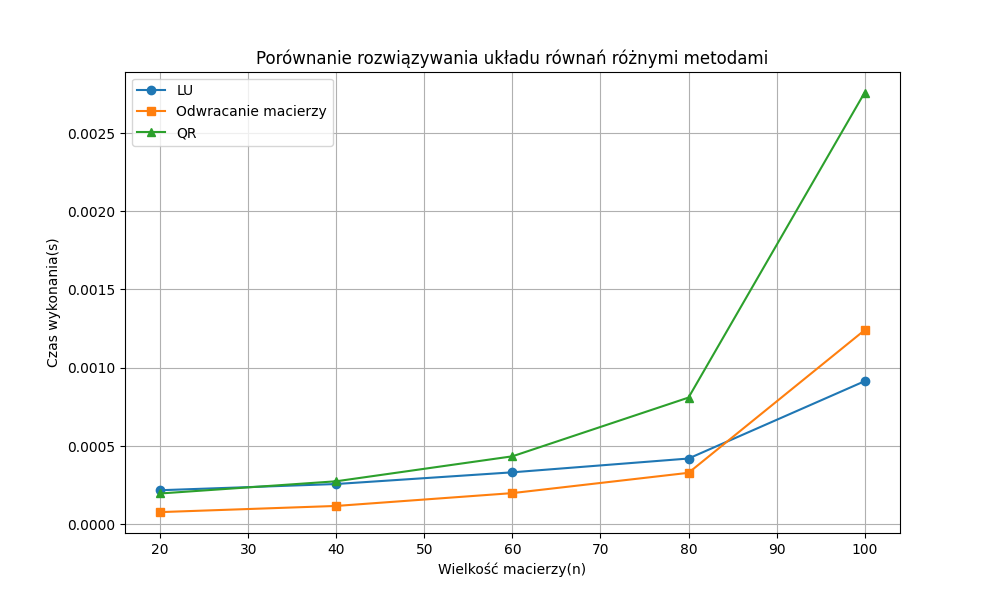
\includegraphics[width=1\linewidth]{Small_values.png}
    \caption{Zależność czasu wykonania od ilości danych dla metod LU, QR i inwersji}
    \label{fig:time_result}
\end{figure}

\subsection{Kod w Python-ie rozwiązujący zadanie}

\begin{lstlisting}
import numpy as np
import time
import matplotlib.pyplot as plt
from random import randrange
import scipy.linalg

def gen_A(n, a=0, b=10):
    return [[randrange(a, b) for _ in range(n)] for _ in range(n)]

def gen_b(n, a=0, b=10):
    return [randrange(a, b) for _ in range(n)]

def solve_inverse_np(A, b):
    A_np = np.array(A)
    b_np = np.array(b)
    
    start = time.time()
    A_inv = np.linalg.inv(A_np)
    x = A_inv @ b_np
    end = time.time()
    
    I1 = A_np @ A_inv
    I2 = A_inv @ A_np
    
    identity = np.eye(len(A))
    is_I1 = np.allclose(I1, identity)
    is_I2 = np.allclose(I2, identity)
    
    print(f"A*A^(-1) = I: {is_I1}")
    print(f"A^(-1)*A = I: {is_I2}")
    
    return x, end - start

def solve_LU(A, b):
    A_np = np.array(A)
    b_np = np.array(b)
    
    start = time.time()
    P, L, U = scipy.linalg.lu(A_np)
    
    y = scipy.linalg.solve_triangular(L, P @ b_np, lower=True)
    
    x = scipy.linalg.solve_triangular(U, y, lower=False)
    end = time.time()
    
    return x, end - start

def solve_QR(A, b):
    A_np = np.array(A)
    b_np = np.array(b)
    
    start = time.time()
    Q, R = np.linalg.qr(A_np)
    
    x = np.linalg.solve(R, Q.T @ b_np)
    end = time.time()
    
    return x, end - start

def verify_solution(A, b, x):
    A_np = np.array(A)
    b_np = np.array(b)
    x_np = np.array(x)
    
    result = A_np @ x_np
    is_correct = np.allclose(result, b_np)
    
    return is_correct

def plot_times(sizes, trials = 100):
    times_lu = []
    times_inv = []
    times_qr = []
    
    for n in sizes:
        sum_time_lu = 0
        sum_time_inv = 0
        sum_time_qr = 0
        for k in range(trials):
            print(f"Calculating for size n={n}")
            A = gen_A(n)
            b = gen_b(n)
            
            _, time_lu = solve_LU(A, b)
            sum_time_lu += time_lu
            
            _, time_inv = solve_inverse_np(A, b)
            sum_time_inv += time_inv
            
            _, time_qr = solve_QR(A, b)
            sum_time_qr += time_qr

        times_lu.append(sum_time_lu/trials)
        times_inv.append(sum_time_inv/trials)
        times_qr.append(sum_time_qr/trials)
    
    plt.figure(figsize=(10, 6))
    plt.plot(sizes, times_lu, 'o-', label='LU')
    plt.plot(sizes, times_inv, 's-', label='Odwracanie macierzy')
    plt.plot(sizes, times_qr, '^-', label='QR')
    plt.xlabel('Wielkość macierzy(n)')
    plt.ylabel('Czas wykonania(s)')
    plt.title('Porównanie rozwiązywania układu równań różnymi metodami')
    plt.legend()
    plt.grid(True)
    plt.show()

def main():
    # n = int(input("Podaj liczbę n (rozmiar układu równań): "))
    n = 10
    A = gen_A(n)
    b = gen_b(n)
    
    print(f"Rozwiązywanie układu {n} równań...")
    
    x_lu, time_lu = solve_LU(A, b)
    is_correct_lu = verify_solution(A, b, x_lu)
    print(f"LU Decomposition: {time_lu:.6f} seconds, solution correct: {is_correct_lu}")
    
    x_inv, time_inv = solve_inverse_np(A, b)
    is_correct_inv = verify_solution(A, b, x_inv)
    print(f"Matrix Inversion: {time_inv:.6f} seconds, solution correct: {is_correct_inv}")
    
    x_qr, time_qr = solve_QR(A, b)
    is_correct_qr = verify_solution(A, b, x_qr)
    print(f"QR Decomposition: {time_qr:.6f} seconds, solution correct: {is_correct_qr}")
    
    print("\Porównanie rozwiązań:")
    print(f"LU i inwersja dają ten sam wynik: {np.allclose(x_lu, x_inv)}")
    print(f"LU i QR dają ten sam wynik: {np.allclose(x_lu, x_qr)}")
    print(f"Inwersja i QR dają ten sam wynik: {np.allclose(x_inv, x_qr)}")
    
    print(f"Generowanie wykresu...")

    sizes = [20 + 20 * i for i in range(5)]
    plot_times(sizes)

if __name__ == "__main__":
    main()
\end{lstlisting}

\section*{Wnioski}

Na podstawie przeprowadzonych eksperymentów można sformułować następujące wnioski:
\begin{itemize}
  \item \textbf{Skuteczność metod:} Wszystkie trzy metody (LU, odwrócenie macierzy, QR) poprawnie wyznaczają rozwiązanie układu równań liniowych, co potwierdza norma reszt (\(\|Ax - b\|_\infty\)) poniżej progu \(10^{-8}\).
  
  \item \textbf{Czas obliczeń:} 
    \begin{enumerate}
      \item \textbf{Dekompzycja LU} okazała się najbardziej wydajna czasowo dla większości rozmiarów macierzy. Jej czas wykonania wzrastał najwolniej, co jest zgodne z teoretyczną analizą złożoności \(\mathcal{O}(n^3)\) z niskim stałym narzutem. Metoda ta uchodzi za optymalną \cite{Rycerz} dla rozwiązywania dużych układów równań z dobrze uwarunkowanymi macierzami.
      
      \item \textbf{Odwracanie macierzy} wykazało zaskakująco dobrą wydajność dla mniejszych rozmiarów (do \(n=80\)), jednak przy większych macierzach (np. \(n=100\)) czas gwałtownie wzrasta, co wynika z kosztownego obliczania odwrotności oraz dodatkowego mnożenia przez wektor. Ta metoda nie powinna być stosowana do rozwiązywania układów równań, ze względu na jej niestabilność i koszt \cite{Rycerz}.
      
      \item \textbf{Dekompozycja QR} była najwolniejsza spośród trzech metod, zwłaszcza dla większych rozmiarów. Dodatkowe koszty wynikają z procesu ortogonalizacji (np. metoda Householdera), co czyni ją mniej efektywną czasowo. Jednakże, QR oferuje lepszą stabilność numeryczną \cite{wiki:Rozkład_QR}, co czyni ją preferowaną metodą w zastosowaniach takich jak regresja liniowa.
    \end{enumerate}
  
  \item Do rozwiązywania dużych układów równań liniowych rekomenduje się dekompozycję LU ze względu na jej efektywność. QR może być wskazane w przypadkach, gdy najważniejsza jest stabilność numeryczna. Odwracanie macierzy należy ograniczyć do sytuacji, gdy rzeczywiście potrzebna jest macierz odwrotna.
  
  \item Uzyskane czasy wykonania były stabilne w kolejnych pomiarach, co świadczy o rzetelności pomiarów i niewielkim wpływie czynników losowych.
\end{itemize}


\bibliographystyle{plain}
\bibliography{references}

\end{document}

